The Computing Platform, mounted on the multirotor, is comprised of two distinct processing platforms: the \textit{Platform Management Board} (PMB) and the \textit{Programmable Logic Board} (PLB). The PMB hosts the software and interfaces required to interface with both the PMB (also present on the multirotor) and the base station.

\begin{figure}[H]\label{hlpic}
    \centering
    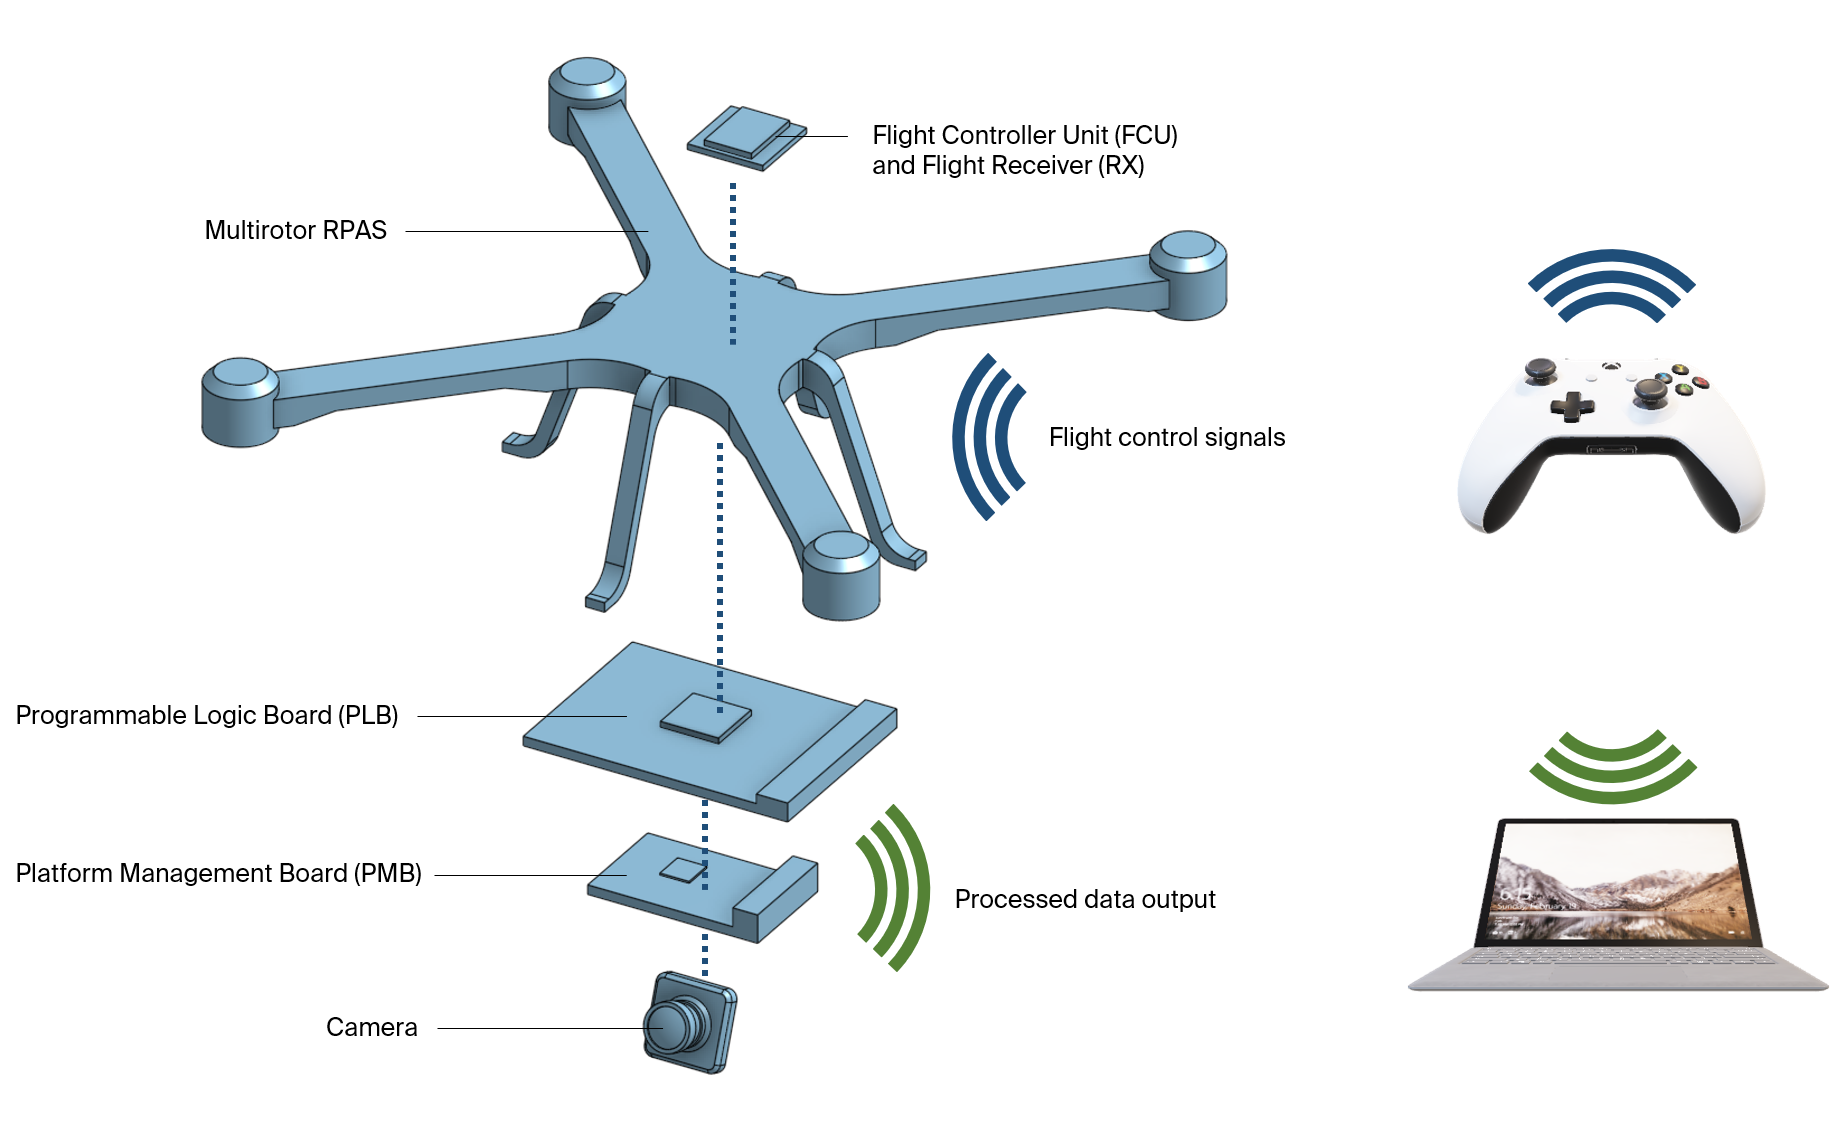
\includegraphics[width=\linewidth]{img/intpic}
\caption{High-Level System Integration with RPAS}
\end{figure}

The multirotor is a quad-engine remote-piloted-aerial system, or multirotor/quadcopter RPAS for short.
The RPAS is propelled electrically using DC sources and motors, and they are controlled by an onboard flight controller unit (FCU) that samples accelerometer data to make fine adjustments to the flight kinematics.
The RPAS is equipped with a receiver to enable flight control via standard radio-control (RC) 2.4 GHz by a pilot.

The RPAS and computing platform are relatively independent since the computing platform provide its own power source. The two modules impose constraints on each other: the computing platform including its power source must be light and compact such that it can be lifted by the RPAS. 
Likewise, the RPAS must provide mounting mechanisms for the computing platform and provide clearance so that equipment are not to be damaged during flight operations.

\begin{figure}[H]\label{hldiag}
\centering
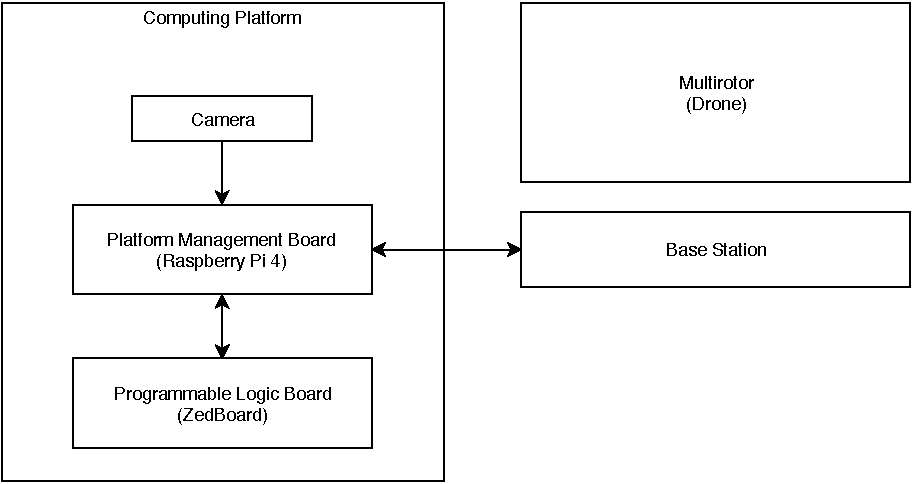
\includegraphics[width=15cm]{img/highlevel.pdf}
\caption{High-Level System Architecture}
\end{figure}

